% !TEX root = ../../AdvStaDaAn.tex
\begin{quote}
\textbf{Statistical (data) analysis} is the science of collecting,
exploring and present (large amounts of) data
to discover underlying patterns
and trends which are \textit{hidden by random noise}.

Many important tasks in statistical data analysis can be expressed
in terms of explaining or modelling the relationship between a response
and one or more explanatory variables or predictors.
\end{quote}
\hfill - Andreas Ruckstuhl
\section{Multiple Linear Regression}
Assume that
\begin{itemize}
\item the response is a continuos variable
\item the explenatory/predictor variables are continuous,
discrete, binary or categorical
\end{itemize}
\begin{align*}
Y_i
=
f(x_i^{(1)},\ldots) + E_i
=
\beta_0 + \beta_1 x_i^{(1)} + \ldots + \beta_m x_i^{(m)}
= \underline{\beta}^T \underline{x_i} + E_i
\end{align*}
The most convenient assumptions are that the random variables $E_i$,
$\forall i=1,\ldots,n$
\begin{itemize}
\item are (stochastically independent)
\item have expectation zero and constant variance $\sigma^2$
(as a function of $i$)
\item are normally (Gaussian) distributed
\end{itemize}

\subsection{Maximum Likelihood Estimation}
\begin{itemize}
\item Maximum likelihood estimation is a method that determines values
for the parameters of a model based on given data.
\item The parameter values are such that they maximise the likelihood that
the process described by the model produced the data that were
actually observed.
\end{itemize}
For linear regression model
\begin{align*}
L(\beta, \sigma | y, X)
=
\frac{1}{(2\pi\sigma^2)^{n/2}}
\exp\left(-\frac{1}{2\sigma^2}(y-X\beta)^T(y-X\beta)\right)
\end{align*}
Maximising the log-likelihood is equivalent to minimizing
$(y-X\beta)^T(y-X\beta)$ if we focus just on $\beta$.
Hence, the OLS estimator $\widehat{\beta}$ is identical to maximum likelihood
estimation.

\subsection{Residuals}
The error terms $E_i$ in the regression model are \textbf{unobservable}.
$\rightarrow$ estimate them by the residuals
\begin{align*}
R
=
Y - X \widehat{\beta}
=
Y - H Y
=
(I - H) Y
, \text{ because }
\widehat{y} =
X \widehat{\beta}
=
X (X^T X)^{-1} X^T Y
\text{ and }
H
\equiv
X (X^T X)^{-1} X^T
\end{align*}
\begin{itemize}
\item \textbf{$R_i$ is normally distributed} since they are a linear
combination of normally distributed random variables.
\item The expectation of the residual is 0
\item The covariance matrix of the residuals is $\sigma^2 (I - H)$
\end{itemize}
\begin{align*}
\text{Scaled residuals}
 &  &
\text{Standardised residuals}
\\
\breve{R_i}
=
\frac{R_i}{\sqrt{1-H_{ii}}}
 &  &
\widetilde{R}_i
=
\frac{R_i}{\sqrt{\widehat{\sigma}^2 (1 - H_{ii})}}
 &  &
\forall i=1,\ldots,n
\end{align*}

\subsection{Prediction}
Predict future values of the response variable for given values of the
predictors.

\textbf{Basic Assumption:} The \textit{estimated} prediction function
represents a true relationship between the variables.

However, there are two sources of uncertainty:
\begin{itemize}
\item The parameters have been estimated
\item The correct functional form is rarely known
\begin{itemize}
\item With an empirically chosen model, the usefulness of prediction is much
less clear
\item We rely on the fact that over limited ranges for the predictors, many
models will behave in nearly the same way
\item so even if we fit the wrong model, we may obtain useful
predictions.
\end{itemize}
\end{itemize}

\subsection{Weighted Least Squares}
Error is now not $\sigma^2$,
but every sample has a different weight $w_i$.
\begin{align*}
Y
=
X \beta + E
,\quad \text{with } E
\sim
\mathbb{N}(0, \sigma^2 W)
,\quad \text{where } W = \text{diag}\left[
\frac{1}{w_1}, \frac{1}{w_2}, \ldots, \frac{1}{w_n}
\right]
\quad \Rightarrow \quad
 &
\widehat{\beta}
=
(X^T W X)^{-1} X^T W Y \\
 &
\widehat{\beta}
\sim
\mathbb{N}\left(\beta, \sigma^2(X^T W X)^{-1}\right)
\end{align*}

\subsection{Robust Fitting}
We remove potential outliers and bad leverage points to get more reliable fits.
Because \textbf{real data} is never exactely Gaussian distributed!
Informal Approach
\begin{enumerate}
\item Examine the data for obvioius outliers
\item Delete the outliers
\item Apply the optimal inference procedure for the assumed model to the
cleaned data set
\end{enumerate}

\subsubsection{Measuring Robustness}
\begin{description}
\item[Gross Error Sensitivity:] Is based on the influence function and
measures the maximum effect of a single observation on the estimated value.
\item[Breakdown Point:] Returns the minimum proportion of data
that can be altered without causing completely unreliable estimates.
\end{description}
Good robustness is when
\begin{itemize}
\item gross error sensitivity is bounded
\item breakdown point of (about) 0.5
\end{itemize}

\subsubsection{M-estimator}
Minimizes
\begin{align*}
\sum_{i=1}^n w_i \cdot r_i \cdot x_i
=
0
\quad
\text{with }
r_i
=
y_i - x_i^T \beta
\end{align*}
Appropriate weights are determined with influence function IF
\begin{align*}
\operatorname{IF}(y)
=
w_i \cdot r_i \cdot M \cdot x_i
\end{align*}
where matrix $M$ only depends on $x_i$.
To limit the influence of leverage points,
one should either
\begin{itemize}
\item be able to identify bad leverage points, or
\item use a re-descending $\psi$-functions
where observations with large absolute residuals are gradually ignored
\end{itemize}

\subsubsection{MM-estimator}
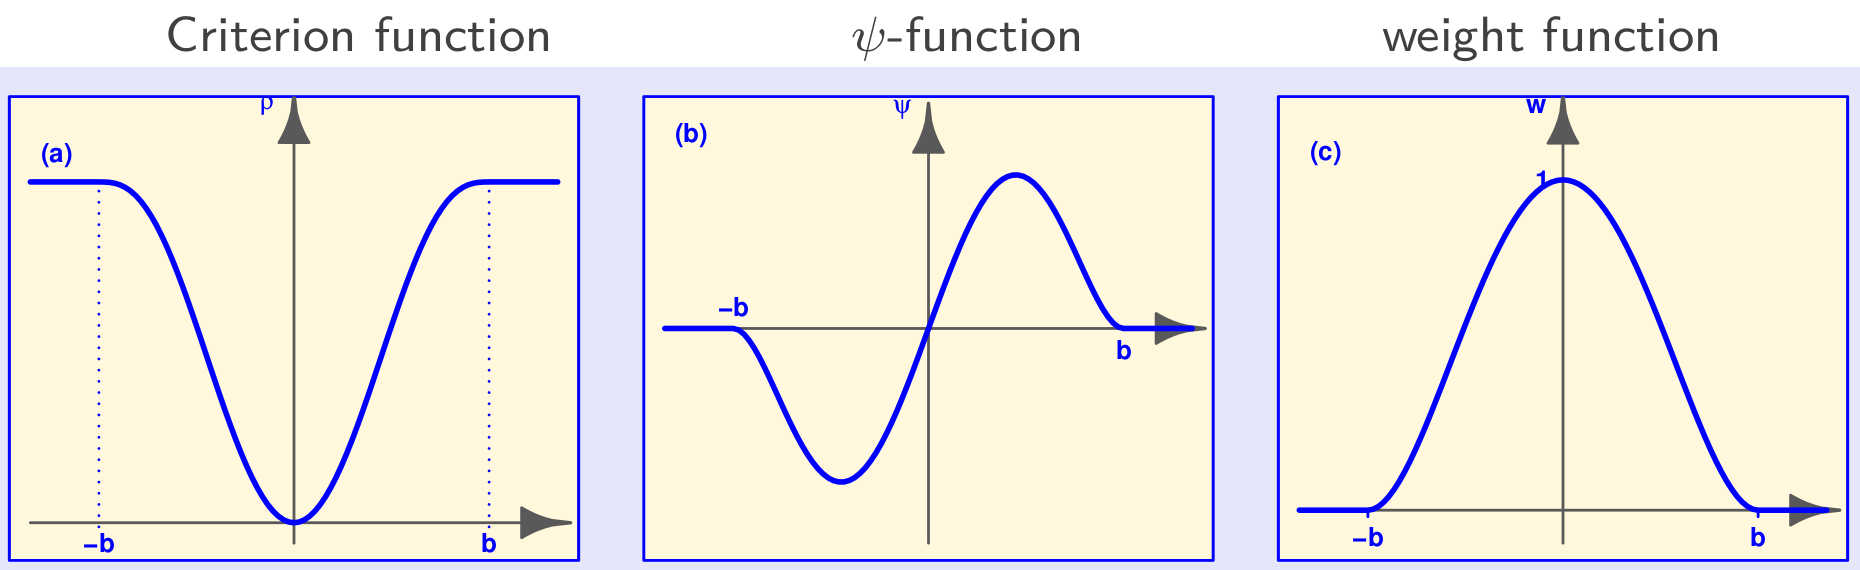
\includegraphics[width=0.7\textwidth]{
sections/MultipleLinearRegression/images/psi-function}
$b$ is fixed at $b=4.687$
\glqq Natural\grqq{} scales for residuales $r_i/\sigma$.
Robust estimator for $\sigma$
\begin{align*}
s_\text{MAV}
=
\frac{\operatorname{median}_i(|r_i|)}{0.6745}
\end{align*}

\subsubsection{Inference}
Covariance matrix $\widehat{V}$ is estimated with
\begin{align*}
 & \widehat{V}
=
s_o^2 \widehat{\tau} \widehat{C}^{-1}
\\
\text{where }
\widehat{C}
=
\frac{1}{n} \frac{\sum_i w_i x_i x_i^T}{\sum_i w_i}
 &             &
\widehat{\tau}
=
\frac{
\frac{1}{n} \sum_{i=1}^n \left( \psi_b \left(\widetilde{r}_i\right)\right)^2
}{
\left(\frac{1}{n} \sum_{i=1}^n \psi_b \left(\widetilde{r}_i\right)\right)^2
}
\\
\text{with }
\widetilde{r}_i
\frac{y_i - x_i^T \widehat{\beta}^{(o)}}{s_o}
 &             &
w_i = \frac{\psi_b(\widetilde{r}_i)}{\widetilde{r}_i}
\end{align*}
note that $\widehat{\beta}^{(o)}$ and
the estimators $s_o$ and $\sigma$ come from the initial estimation.